The next step is to find the inverse kinematic (IK) solution for the right arm.
Inherently this problem has multiple solutions.
When solving the IK Pieper\cite{peiper1968kinematics} states that a closed-form solution does exist if:
\begin{itemize}
\item Three consecutive joints axes of the manipulator are parallel to one another
\end{itemize}

OR
\begin{itemize}
\item Three consecutive joints intercect at a single point
\end{itemize}

The kinematic structure in Fig~\ref{fig:hubo} and Fig~\ref{fig:IkFkCoordinate} shows that the Hubo2+ platform does have a three joints that intersect the same point in the shoulders and in the hips.
Thus a closed-form solution exists for both arms and both legs.

The transform $T_0^6$ in Equation~\ref{eq:t06} is needed to solve the IK problem for the shoulder.  
It is important to note that $T_0^6$ is in the form of

\begin{equation}\label{eq:T06}
T_0^6 = \left[ \begin{array}{cccc} 
\overline{x_6} & \overline{y_6} & \overline{z_6} & \overline{p_6} \\
0              & 0              & 0              & 1   
\end{array} \right]
\end{equation} 

Where $\overline{x_6}$, $\overline{y_6}$ and $\overline{z_6}$ are $[3x1]$ unit vectors along the principle axes of the end-effectors coordinate frame $i$, see Fig.~\ref{fig:IkFkCoordinate}.
Position vector $\overline{p_6}$ describes the hand about joint $A1$ (shoulder).
The arm can be vied in different frames.
If we look at the arm in reference to the end-effector's frame.
The reverse transform is defined as $(T_0^6)`$


\begin{equation}
(T_0^6)' = T_6^0 = (T_0^6)^{-1} = \left[ \begin{array}{cccc} 
\overline{x_6} & \overline{y_6} & \overline{z_6} & \overline{p_6} \\
0              & 0              & 0              & 1   
\end{array} \right]^{-1}
\end{equation} 

The following method is based on the work done by our partner Park et. al.\cite{5649842}.
The general link translation matrix $T_{i-1}^i$ relates the $i^{th}$ coordinate frame to the $(i-1)^{th}$ coordinate frame.  
In addition we can extend Equation~\ref{eq:T06} to

\begin{equation}\label{eq:06invIK}
T_0^6 = \left[ \begin{array}{cccc} 
\overline{x_6} & \overline{y_6} & \overline{z_6} & \overline{p_6} \\
0              & 0              & 0              & 1   
\end{array} \right] = \left[ \begin{array}{cccc} 
\overline{n} & \overline{s} & \overline{a} & \overline{p} \\
0            & 0            & 0            & 1   
\end{array} \right]
\end{equation} 

Where $[\overline{n}, \overline{s}, \overline{a}, \overline{p}]$ represents the normal vector, the sliding vector, the approach vector and the position vector of the end effector respectively\cite{fu1987robotics}.  We can now state that

\begin{equation}
(T_0^6)' = T_6^0 = (T_0^6)^{-1} = \left[ \begin{array}{cccc} 
\overline{x_6} & \overline{y_6} & \overline{z_6} & \overline{p_6} \\
0              & 0              & 0              & 1   
\end{array} \right]^{-1}= \left[ \begin{array}{cccc} 
\overline{n}' & \overline{s}' & \overline{a}' & \overline{p}' \\
0             & 0             & 0             & 1   
\end{array} \right]
\end{equation} 

We can now use the reverse method to solve for the joint angles as in \cite{fu1987robotics} and derived in the tech report\cite{gtechIK2}.
The first three lower joint angles of $A_4$, $A_5$ and $A_6$ are solved for.
Subsequently the upper joint angles of $A_1$, $A_2$ and $A_3$ are solved.

Using inverse transform methods\cite{4046335} we can modify Equation~\ref{eq:t06} to

\begin{equation}\label{eq:t06IK}
T_6^0 = (T_0^6)^{-1} = \prod_{i=6}^{1} T_{i}^{i-1} = T_{6}^{5}T_{5}^{4}T_{4}^{3}T_{3}^{2}T_{2}^{1}T_{1}^{0}
\end{equation}

Then we equate Equation~\ref{eq:06invIK} to Equation~\ref{eq:t06IK} 

\begin{equation}
T_{6}^{5}T_{5}^{4}T_{4}^{3}T_{3}^{2}T_{2}^{1}T_{1}^{0} = \left[ \begin{array}{cccc} 
\overline{n}' & \overline{s}' & \overline{a}' & \overline{p}' \\
0             & 0             & 0             & 1   
\end{array} \right]
\end{equation}

Then move $T_6^5$ to the other side of the equation


\begin{equation}\label{eq:preG}
T_{5}^{4}T_{4}^{3}T_{3}^{2}T_{2}^{1}T_{1}^{0} = T_{5}^{6}\left[ \begin{array}{cccc} 
\overline{n}' & \overline{s}' & \overline{a}' & \overline{p}' \\
0             & 0             & 0             & 1   
\end{array} \right]
\end{equation}

For simplicity we will represent Equation~\ref{eq:preG} as $G_L$ and $G_R$ standing for \textit{right} and \textit{left} side.

\begin{equation}
G_L = T_{5}^{6}\left[ \begin{array}{cccc} 
\overline{n}' & \overline{s}' & \overline{a}' & \overline{p}' \\
0             & 0             & 0             & 1   
\end{array} \right]
\end{equation}



\begin{equation}
G_R = T_{5}^{4}T_{4}^{3}T_{3}^{2}T_{2}^{1}T_{1}^{0} 
\end{equation}


Expanding gives us

\begin{equation}
G_L = \left[ \begin{array}{cccc} 
g_{11} & g_{12} & g_{13} & cos(\theta_6)(p_x'+l_{A_4})-sin(\theta_6)p_y' \\
g_{21} & g_{22} & g_{23} & sin(\theta_6)(p_x'+l_{A_4})-cos(\theta_6)p_y' \\
g_{31} & g_{32} & g_{33} & p_z'                                         \\
0      & 0      & 0      & 1   
\end{array} \right]
\end{equation}

and

\begin{equation}
G_R = \left[ \begin{array}{cccc} 
g_{11} & g_{12} & g_{13} & sin(\theta_4)cos(\theta_5)l_{A_2} \\
g_{21} & g_{22} & g_{23} & -cos(\theta_6)l_{A_2}-l_{A3}       \\
g_{31} & g_{32} & g_{33} & sin(\theta_4)sin(\theta_5)l_{A_2}  \\
0      & 0      & 0      & 1   
\end{array} \right]
\end{equation}

We can then equate elements $(1,4)$, $(2,4)$ and $(3,4)$ of $G_L$ and $G_R$. 
This gives us

\begin{equation}\label{eq:thetaSolve11}
cos(\theta_6)(p_x'+l_{A_4})-sin(\theta_6)p_y' = sin(\theta_4)cos(\theta_5)l_{A_2}
\end{equation}

\begin{equation}\label{eq:thetaSolve12}
sin(\theta_6)(p_x'+l_{A_4})-cos(\theta_6)p_y' = -cos(\theta_6)l_{A_2}-l_{A3}
\end{equation}

\begin{equation}\label{eq:thetaSolve13}
p_z' = sin(\theta_4)sin(\theta_5)l_{A_2}
\end{equation}

Based on the desired task space location we let

\begin{equation}\label{eq:thetaSolve21}
p_x' + l_{A_4} = r \cdot cos(\phi)
\end{equation}

and

\begin{equation}\label{eq:thetaSolve22}
p_y' = r \cdot sin(\phi)
\end{equation}

where 

\begin{equation}\label{eq:thetaSolve31}
r = sqrt{(p_x'+l_{A_4})^2 + (p_y')^2}
\end{equation}

and 

\begin{equation}\label{eq:thetaSolve32}
\phi = atan2(p_y',p_x'+l_{A_4})
\end{equation}

\textbf{Note:} $atan2()$ represents the the $atan$ method that gathers the information of the signs of the inputs in order to put the returned value in the appropriate quadrant.

Combining Equation (\ref{eq:thetaSolve11}), (\ref{eq:thetaSolve12}) and (\ref{eq:thetaSolve13}) with Equation (\ref{eq:thetaSolve21}) and (\ref{eq:thetaSolve22}) we get

\begin{equation}\label{eq:thetaSolve41}
r \cdot cos(\theta_6+\phi) = sin(\theta_4)cos(\theta_5)l_{A_2}
\end{equation}

\begin{equation}\label{eq:thetaSolve42}
r \cdot sin(\theta_6+\phi) = -cos(\theta_4)l_{A_2}-l_{A_3}
\end{equation}

\begin{equation}\label{eq:thetaSolve43}
p_z' = sin(\theta_4)sin(\theta_5)l_{A_2}
\end{equation}


When we combine above with Equation (\ref{eq:thetaSolve31}) and (\ref{eq:thetaSolve32}) and obtain 


\begin{equation}
\theta_4 = atan2\left( \pm \sqrt{1-cos(\theta_4)^2} , cos(\theta_4)  \right)
\end{equation}

where

\begin{equation}
cos(\theta_4) = \frac{(p_x'+l_{A_4})^2  +  p_y'^2  +  p_z'^2  -  l_{A_2}^2  -  l_{A_3}^2}
                     {2l_{A_2}l_{A3}}
\end{equation}

Using Equation~\ref{eq:thetaSolve43} we can get $\theta_5$

\begin{equation}
\theta_5 = atan2(sin(\theta_5), \pm\sqrt{1-sin(\theta_5)^2})
\end{equation}

where

\begin{equation}
sin(\theta_5) = \frac{p_z'}
                     {sin(\theta_4)l_{A_2}}
\end{equation}


We can then solve for $\theta_6$ by dividing Equation~\ref{eq:thetaSolve42} by Equation~\ref{eq:thetaSolve41}.



\begin{equation}
\frac{r \cdot sin(\theta_6+\phi)}
     {r \cdot cos(\theta_6+\phi)} = tan(\theta_6+\phi) = \frac{-cos(\theta_4)l_{A_2}-l_{A_3}}
                                                              {sin(\theta_4)cos(\theta_5)l_{A_2}}
\end{equation}

\begin{equation}
\theta_6 = atan2(-(cos(\theta_4)l_{A_2}+l_{A_3}), sin(\theta_4)cos(\theta_5)l_{A_2}) - \phi
\end{equation}


Now that we have $\theta_4$, $\theta_5$ and $\theta_6$ we reconstruct $G$ in reference to joint $A_1$, $A_2$ and $A_3$.  We will call this $G^*$.  Like $G$ we will have a right ($G^*_R$) and left ($G^*_R$) of $G$:

\begin{equation}
G_L^* = \left[ \begin{array}{cccc} 
g_{11}^* & g_{12}^* & g_{13}^* & g_{14}^* \\
g_{21}^* & g_{22}^* & g_{23}^* & g_{24}^* \\
g_{31}^* & g_{32}^* & g_{33}^* & g_{34}^* \\
0        & 0        & 0        & 1   
\end{array} \right]
\end{equation}

\scriptsize
\begin{equation}
G_R^* = \left[ \begin{array}{cccc} 
cos(\theta_1)cos(\theta_2)cos(\theta_3)-sin(\theta_1)sin(\theta_3) & cos(\theta_1)sin(\theta_3) + sin(\theta_1)cos(\theta_2)cos(\theta_3) & sin(\theta_2)cos(theta_3) & 0 \\
-cos(\theta_1)sin(\theta_2) & -sin(\theta_1)sin(\theta_1) & cos(\theta_2) & l_{A_2} \\
sin(\theta_1)cos(\theta_3)+cos(\theta_1)cos(\theta_2)sin(\theta_3) & sin(\theta_1)cos(\theta_2)sin(\theta_3)-cos(\theta_1)cos(\theta_3) & sin(\theta_2)sin(\theta_3) & 0 \\
0        & 0        & 0        & 1   
\end{array} \right]
\end{equation}
\normalsize

as before we can copare the elements of $G^*_L$ and $G^*_R$.  
Specifically compare element $(2,3)$.
We then get

\begin{equation}
cos(\theta_2) = \begin{array}{l} a_z'sin(\theta_4)sin(\theta_5) - a_y'(cos(\theta_4)cos(\theta_6) + sin(\theta_4)cos(\theta_5)sin(\theta_6)) \\
-a_x'(cos(\theta_4)sin(\theta_6)-sin(\theta_4)cos(\theta_5)cos(\theta_6))
\end{array}
\end{equation}

\begin{equation}
\theta_2 = atan2(\pm \sqrt{1-cos(\theta_2)^2}, cos(\theta_2))
\end{equation}

If we take elements $(1,3)$ and $(3,3)$ of $G^*_L$ with those of $G^*_R$ we get

\begin{equation}
g^*_{13} = \begin{array}{l} a_x'( cos(\theta_4)cos(\theta_5)cos(\theta_6) + sin(\theta_4)sin(\theta_6) + a_z'cos(\theta_4)sin(\theta_5) \\
+ a_y'(sin(\theta_4)cos(\theta_6)-cos(\theta_4)cos(\theta_5)sin(\theta_6))
\end{array}
\end{equation}

By dividing these two equations we can get $\theta_1$

\begin{equation}
\theta_2 = atan2(g^*_{33}, g^*_{13})
\end{equation}

and thus

\begin{equation}
\begin{array}{rcrc}IF:& sin(\theta_2)<0 & THEN: & \theta_1 = \theta_1 + \pi
\end{array}
\end{equation}

Fig.~\ref{fig:6dofik} shows the example of using Hubo-Ach to move the right end-effector to the desired work space coordinates using the IK method described in this section.

\begin{figure}[thpb]
  \centering
      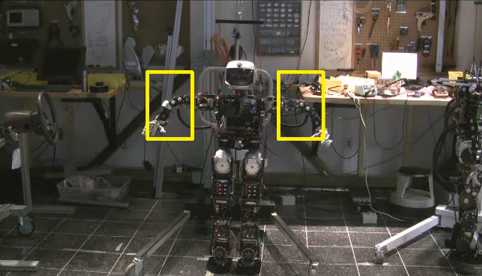
\includegraphics[width=0.69\columnwidth]{./pix/6dofik2hands.png}
      
\includegraphics[width=0.3\columnwidth]{./qrcode/qrcode-6dofik.png}\\
      Video: http://danlofaro.com/phd/ik/\#HuboTwoArmIk
\caption{Hubo preforming 6-DOF IK in real-time using method discussed in Section~\ref{sec:ik}}
\label{fig:6dofik}
\end{figure}
